\documentclass[a4paper,12pt]{article}
\usepackage{graphicx}
\usepackage{booktabs}
\usepackage{array}

\textheight=24.3cm
\topmargin=-1.8cm
\textwidth=16.7cm
\oddsidemargin=-0.3cm
\evensidemargin=0.0cm
\parindent=0pt
\parskip=6pt

\begin{document}

\section*{2.1}

\textbf{a)}\par\nopagebreak
\begin{tabular}{>{\raggedright\arraybackslash}p{3.3cm}
  *{2}{>{\raggedright\arraybackslash}p{6cm}}}
\toprule
 & PCA dimension reduction & Spectral embedding \\
\midrule
optimization goal & maximize the variance of the data projected onto $k$
  orthogonal directions & minimize $\sum_{i,j}w_{ij}\|y_i-y_j\|^2
  =2\,\mathrm{tr}(Y^TLY)$ subject to $Y^TY=I$ \\
matrix for the eigendecomposition & covariance matrix
  $C=\frac{1}{n-1}D^TD$ of the mean-centred $D$ & Laplacian $L=\Lambda-W$
  of the similarity graph \\
size of the matrix & $d\times d$ & $n\times n$ \\
$k$ best eigenvalues & $\lambda_{\max-k+1},\dots,\lambda_{\max}$ (largest)
  & $\lambda_2,\dots,\lambda_{k+1}$ (smallest except $\lambda_1=0$) \\
new data after transformation & $DP_k$ with
  $P_k=[v_{\max-k+1},\dots,v_{\max}]$ ($n\times k$) &
  $[v_2,\dots,v_{k+1}]$ ($n\times k$) \\
\bottomrule
\end{tabular}

\textbf{b)} $\sqrt{53}=d((0,0),(7,-2))$ is the largest distance between two
points, so the similarities lie in $[0,1]$. With the points numbered 1--6
in the given order, the 2-nearest neighbour graph has the edges 1--2, 2--3,
4--5 and 5--6 with similarity 0.717, 1--4 with 0.566, 2--4 with 0.752,
3--4 with 0.693 and 4--6 with 0.434.
\[
L=\left(\begin{array}{rrrrrr}
1.282 & -0.717 & 0 & -0.566 & 0 & 0\\
-0.717 & 2.186 & -0.717 & -0.752 & 0 & 0\\
0 & -0.717 & 1.410 & -0.693 & 0 & 0\\
-0.566 & -0.752 & -0.693 & 3.161 & -0.717 & -0.434\\
0 & 0 & 0 & -0.717 & 1.434 & -0.717\\
0 & 0 & 0 & -0.434 & -0.717 & 1.150
\end{array}\right)
\]
has the eigenvalues $0,\,0.598,\,1.342,\,1.993,\,2.851,\,3.839$ with the
eigenvectors in the columns of
\[
V=\left(\begin{array}{rrrrrr}
0.408 & 0.390 & 0.711 & -0.044 & 0.399 & 0.120\\
0.408 & 0.344 & -0.027 & -0.039 & -0.796 & 0.282\\
0.408 & 0.334 & -0.700 & -0.076 & 0.443 & 0.173\\
0.408 & 0.036 & -0.041 & 0.105 & -0.098 & -0.900\\
0.408 & -0.493 & 0.013 & 0.727 & 0.047 & 0.244\\
0.408 & -0.611 & 0.043 & -0.672 & 0.005 & 0.080
\end{array}\right).
\]
The 1-dimensional presentation is
$v_2=(0.390,\,0.344,\,0.334,\,0.036,\,-0.493,\,-0.611)$. It preserves the
clustering structure: points 1--3 lie together at 0.33--0.39 and points 4--6
below them, although point 4 lies between the clusters.

\textbf{c)} The PCA presentation orders the points 1, 2, 4, 3, 5, 6, so
point 4 falls between points 2 and 3 and the clusters overlap, whereas the
spectral embedding keeps them apart. PCA keeps the direction of largest
variance and ignores which points are neighbours. Here $v_1$ runs along both
elongated clusters, while the clusters are separated in a direction of small
variance that is discarded.

\begin{center}
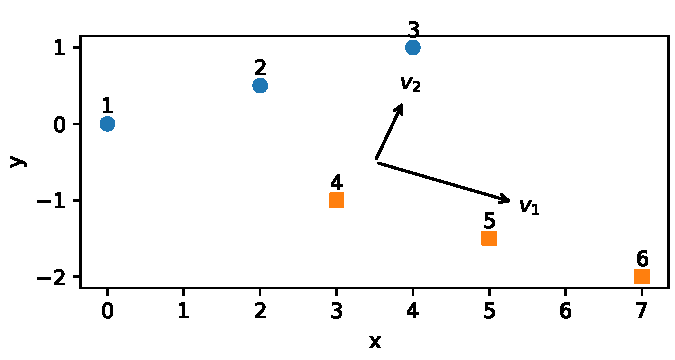
\includegraphics[width=0.6\textwidth]{figures/pca.pdf}
\end{center}

\section*{2.2}

\textbf{1.}\par\nopagebreak
\begin{tabular}{lcccccccccrr}
\toprule
 & & \multicolumn{8}{c}{Label of point} & \multicolumn{2}{c}{Representative} \\
\cmidrule(lr){3-10}\cmidrule(lr){11-12}
Run & Iteration & 1 & 2 & 3 & 4 & 8 & 10 & 11 & 100 & $c_1$ & $c_2$ \\
\midrule
K-Means, (8), (11) & 1 & 1 & 1 & 1 & 1 & 1 & 2 & 2 & 2 & 3.6 & 40.33 \\
 & 2 & 1 & 1 & 1 & 1 & 1 & 1 & 1 & 2 & 5.57 & 100 \\
 & 3 & 1 & 1 & 1 & 1 & 1 & 1 & 1 & 2 & 5.57 & 100 \\
\midrule
K-Means, (1), (8) & 1 & 1 & 1 & 1 & 1 & 2 & 2 & 2 & 2 & 2.5 & 32.25 \\
 & 2 & 1 & 1 & 1 & 1 & 1 & 1 & 1 & 2 & 5.57 & 100 \\
 & 3 & 1 & 1 & 1 & 1 & 1 & 1 & 1 & 2 & 5.57 & 100 \\
\midrule
K-Medians, (8), (11) & 1 & 1 & 1 & 1 & 1 & 1 & 2 & 2 & 2 & 3 & 11 \\
 & 2 & 1 & 1 & 1 & 1 & 2 & 2 & 2 & 2 & 2.5 & 10.5 \\
 & 3 & 1 & 1 & 1 & 1 & 2 & 2 & 2 & 2 & 2.5 & 10.5 \\
\midrule
K-Medians, (1), (8) & 1 & 1 & 1 & 1 & 1 & 2 & 2 & 2 & 2 & 2.5 & 10.5 \\
 & 2 & 1 & 1 & 1 & 1 & 2 & 2 & 2 & 2 & 2.5 & 10.5 \\
\midrule
K-Medians, (1), (100) & 1 & 1 & 1 & 1 & 1 & 1 & 1 & 1 & 2 & 4 & 100 \\
 & 2 & 1 & 1 & 1 & 1 & 1 & 1 & 1 & 2 & 4 & 100 \\
\bottomrule
\end{tabular}

K-Means ends with $\{1,\dots,11\}$ and $\{100\}$ from both initializations,
because the outlier pulls the mean of its cluster away. K-Medians is more
robust to the outlier and finds $\{1,2,3,4\}$ and $\{8,10,11,100\}$, unless
the outlier is an initial representative, in which case it stays a
singleton cluster as with K-Means. The result thus depends on the algorithm
and the initialization, and an outlier can take a whole cluster.

\textbf{2.}\par\nopagebreak
\begin{tabular}{rrrrrrr}
\toprule
 & \multicolumn{3}{c}{\#1} & \multicolumn{3}{c}{\#2} \\
\cmidrule(lr){2-4}\cmidrule(lr){5-7}
$x$ & $a$ & $b$ & $S(x)$ & $a$ & $b$ & $S(x)$ \\
\midrule
1 & 2.00 & 31.25 & 0.936 & 5.33 & 99.00 & 0.946 \\
2 & 1.33 & 30.25 & 0.956 & 4.50 & 98.00 & 0.954 \\
3 & 1.33 & 29.25 & 0.954 & 4.00 & 97.00 & 0.959 \\
4 & 2.00 & 28.25 & 0.929 & 3.83 & 96.00 & 0.960 \\
8 & 32.33 & 5.50 & $-0.830$ & 4.50 & 92.00 & 0.951 \\
10 & 31.00 & 7.50 & $-0.758$ & 5.50 & 90.00 & 0.939 \\
11 & 31.00 & 8.50 & $-0.726$ & 6.33 & 89.00 & 0.929 \\
100 & 90.33 & 97.50 & 0.074 & & & 0 \\
\midrule
$SC$ & & & 0.192 & & & 0.830 \\
\bottomrule
\end{tabular}

No. SC prefers \#2, but the outlier is so far away that it dominates the
mean distances. In \#2 all other points get $S\approx0.95$ although the
groups $\{1,2,3,4\}$ and $\{8,10,11\}$ are merged, and in \#1 the points 8,
10 and 11 get negative silhouettes although they form a natural group.

\section*{2.3}

\textbf{a)} Clusters and classes coincide, so $I(C,D)=H(C)=H(D)=1$ bit and
$NMI=1$.

\textbf{b)} Each cluster contains one point of each class, so
$P(C_i,D_j)=\frac14=P(C_i)P(D_j)$, $I(C,D)=0$ and $NMI=0$.

\textbf{c)} $H(C)=2$ bits and $H(D)=1$ bit, and every singleton cluster is
pure, so $I(C,D)=H(D)=1$ bit and $NMI=1/\sqrt2\approx0.71$. This is not
intuitive, because the classes are irrelevant to the clustering.

\textbf{d)} Independence holds for the true probabilities, but NMI is
computed from relative frequencies in the data. With singleton clusters,
$P(C_i,D_j)=1/n$ for the class of the point and 0 otherwise, which never
equals $P(C_i)P(D_j)=P(D_j)/n$. The estimated mutual information is
therefore always $H(D)>0$, and this bias grows with the number of clusters.

\end{document}
